% =============================================================================
% Module 6: Fermat's Principle and Time Delays
% =============================================================================
% Sources: Saha et al. Sec. 1.2-1.3, Narayan & Bartelmann Sec. 3.3,
%          Congdon & Keeton Ch. 4.3-4.4
% Mathematica: ../Mathematica/06_Fermat_Time_Delays/
% =============================================================================

\chapter{Fermat's Principle and Time Delays}
\label{ch:fermat_time_delays}

\begin{quote}
\textit{The positions of the images of a gravitational lens are determined
by Fermat's principle: images form at stationary points of the arrival
time.  The time delays between multiple images, in turn, give us a
direct measurement of cosmological distances --- and hence the Hubble
constant.}
\hfill --- Narayan \& Bartelmann (1997)
\end{quote}

\noindent
In Module~\ref{ch:lens_equation} we derived the lens equation
$\vecbeta = \vectheta - \vecalpha(\vectheta)$ as a geometric
consequence of light deflection.  In Module~\ref{ch:light_deflection}
we computed the Shapiro time delay experienced by photons passing
through a gravitational potential, and in
Module~\ref{ch:linearized_gravity} we introduced the effective
refractive index of a weak gravitational field.

In this module we show that the lens equation itself emerges from a
variational principle: images form at stationary points of the
\textbf{arrival-time surface}.  This elegant reformulation ---
Fermat's principle for gravitational lensing --- not only provides a
deeper understanding of image formation, but also yields
\textbf{observable time delays} between multiple images.  These time
delays are directly proportional to $\Hubble^{-1}$, making
multiply-imaged variable sources (such as quasars) a powerful and
independent probe of the Hubble constant.

\medskip
\noindent
\textbf{Companion Mathematica files:}
\begin{itemize}[nosep]
    \item \mathlink{06_Fermat_Time_Delays/time_delay_function.wl}{time\_delay\_function.wl}
          --- symbolic computation of the Fermat potential, verification
          that $\nabla\tau = 0$ recovers the lens equation, time delay
          formulas for point mass and SIS lenses, numerical $\Hubble$
          estimation, and publication-quality figure generation
    \item \mathlink{06_Fermat_Time_Delays/arrival_time_surface.nb}{arrival\_time\_surface.nb}
          --- interactive notebook: 3D arrival-time surface with slider
          for source position, contour plots with critical curves,
          time delay visualization
\end{itemize}


% =====================================================================
\section{Introduction: From Geometry to a Variational Principle}
\label{sec:fermat_intro}

The lens equation $\vecbeta = \vectheta - \vecalpha(\vectheta)$ was
derived in Module~\ref{ch:lens_equation} by tracing light rays through
the lensing geometry.  While this approach is direct and intuitive, it
does not explain \textit{why} light ``chooses'' particular paths through
the lens plane, nor does it immediately reveal the relative arrival times
of multiple images.

A deeper perspective comes from \textbf{Fermat's principle}: among all
possible paths from source to observer, light follows those for which the
travel time is \textit{stationary} (a minimum, maximum, or saddle point
of the arrival time).  In classical optics, Fermat's principle explains
Snell's law and the focusing properties of lenses.  In gravitational
lensing, it does far more:
\begin{enumerate}
    \item It \textbf{derives} the lens equation as the stationarity
          condition $\nabla_{\vectheta}\, t = 0$.
    \item It \textbf{classifies} multiple images by the nature of the
          stationary point (minimum, saddle, or maximum), which
          determines their parity and arrival order.
    \item It produces \textbf{observable time delays} between multiple
          images, which can be used to measure the Hubble constant.
\end{enumerate}

The key quantity is the \textbf{time delay function} (or
\textbf{arrival-time surface}) $t(\vectheta)$, which gives the arrival
time of a photon traveling from a source at $\vecbeta$ via the lens
plane at $\vectheta$ to the observer.  Images form at the stationary
points of $t(\vectheta)$, and the differences in $t$ between stationary
points give the time delays.


% =====================================================================
\section{The Time Delay Function}
\label{sec:time_delay_function}

Consider a photon emitted by a source at angular position $\vecbeta$ in
the source plane.  The photon passes through the lens plane at angular
position $\vectheta$ and arrives at the observer.  The total travel time
relative to the unperturbed (unlensed, straight-line) path consists of
two contributions:

\begin{itemize}
    \item \textbf{Geometric delay} (extra path length): The deflected ray
          travels a longer geometric path than the straight-line ray.  In
          the small-angle, thin-lens approximation, the extra path length
          corresponds to an angular excess of $\half|\vectheta - \vecbeta|^2$
          (see Module~\ref{ch:lens_equation}, Section~\ref{sec:lensing_geometry}).
    \item \textbf{Shapiro (gravitational) delay}: The photon passes
          through the gravitational potential of the lens, experiencing the
          time delay derived in Module~\ref{ch:light_deflection}.  In the
          thin-lens formalism, this delay is encoded in the
          \textbf{lensing potential} $\psiL(\vectheta)$
          (Module~\ref{ch:magnification_convergence_shear}).
\end{itemize}

Combining these contributions, the total arrival time is
(Narayan \& Bartelmann eq.~21; Congdon \& Keeton eq.~4.46):
\begin{equation}
    \boxed{
    t(\vectheta) = \frac{(1 + z_d)}{\speedoflight}\,
    \frac{\Dd\,\Ds}{\Dds}\,
    \left[\half|\vectheta - \vecbeta|^2 - \psiL(\vectheta)\right]
    + \text{const}
    }
    \label{eq:time_delay_function}
\end{equation}
where $z_d$ is the redshift of the lens, the angular diameter distances
$\Dd$, $\Ds$, $\Dds$ are defined in Module~\ref{ch:cosmological_distances},
and the constant is an irrelevant additive term that depends on the
unperturbed travel time.

The factor $(1 + z_d)$ converts from the lens-frame time to the
observer-frame time (cosmological time dilation).  The combination
$\Dd\,\Ds / \Dds$ is the \textbf{effective lensing distance}, which
encodes the geometry of the observer--lens--source system.

\begin{definition}[Fermat potential]
The dimensionless quantity
\begin{equation}
    \boxed{
    \tau(\vectheta, \vecbeta) = \half|\vectheta - \vecbeta|^2
    - \psiL(\vectheta)
    }
    \label{eq:fermat_potential}
\end{equation}
is called the \textbf{Fermat potential} (or \textbf{time delay
potential}).  The arrival time is proportional to $\tau$:
\begin{equation}
    t(\vectheta) = \frac{(1 + z_d)}{\speedoflight}\,
    \frac{\Dd\,\Ds}{\Dds}\, \tau(\vectheta, \vecbeta)
    + \text{const} \,.
    \label{eq:t_tau_relation}
\end{equation}
\end{definition}

\begin{remark}
The Fermat potential has a simple physical interpretation:
\begin{itemize}[nosep]
    \item The first term $\half|\vectheta - \vecbeta|^2$ is the
          \textbf{geometric delay}: it penalizes paths where the ray in the
          lens plane ($\vectheta$) is far from the straight-line direction
          ($\vecbeta$).
    \item The second term $-\psiL(\vectheta)$ is the
          \textbf{gravitational (Shapiro) delay}: the lensing potential
          $\psiL > 0$ in the vicinity of the lens, so this term
          \textit{reduces} the arrival time --- photons passing through a
          deeper potential arrive earlier due to the Shapiro effect
          (recall Module~\ref{ch:light_deflection}).
\end{itemize}
The competition between geometric and gravitational delay determines the
structure of the arrival-time surface and hence the number and types of
images.
\end{remark}


% =====================================================================
\section{Fermat's Principle and the Lens Equation}
\label{sec:fermat_principle}

\textbf{Fermat's principle} states that images form at stationary points
of the arrival time $t(\vectheta)$, or equivalently, at stationary points
of the Fermat potential $\tau(\vectheta, \vecbeta)$:
\begin{equation}
    \nabla_{\vectheta}\, t(\vectheta) = 0
    \quad \Longleftrightarrow \quad
    \nabla_{\vectheta}\, \tau(\vectheta, \vecbeta) = 0 \,.
    \label{eq:fermat_condition}
\end{equation}

Computing the gradient of $\tau$:
\begin{align}
    \nabla_{\vectheta}\, \tau &= \nabla_{\vectheta}\left[
    \half|\vectheta - \vecbeta|^2 - \psiL(\vectheta)\right]
    \nonumber \\
    &= (\vectheta - \vecbeta) - \nabla\psiL(\vectheta) \,.
    \label{eq:grad_tau}
\end{align}
Setting this to zero:
\begin{equation}
    \vectheta - \vecbeta - \nabla\psiL(\vectheta) = 0
    \qquad \Longrightarrow \qquad
    \vecbeta = \vectheta - \nabla\psiL(\vectheta) \,.
    \label{eq:lens_eq_from_fermat}
\end{equation}
Since the reduced deflection angle is $\vecalpha(\vectheta) = \nabla\psiL(\vectheta)$
(from Module~\ref{ch:magnification_convergence_shear}), this is precisely
the \textbf{lens equation}:
\begin{equation}
    \boxed{
    \vecbeta = \vectheta - \vecalpha(\vectheta)
    }
    \label{eq:lens_eq_fermat}
\end{equation}

\begin{remark}
This is a remarkable result: the lens equation, which we previously derived
from ray-tracing geometry, follows directly from the
\textbf{stationarity of the arrival time}.  Fermat's principle provides
a variational derivation of the fundamental equation of gravitational
lensing.  The connection between the gradient of the lensing potential and
the deflection angle, $\vecalpha = \nabla\psiL$, was established in
Module~\ref{ch:magnification_convergence_shear} from the Poisson equation
$\nabla^2\psiL = 2\kappab$.
\end{remark}


% =====================================================================
\section{Classification of Images: Morse Theory}
\label{sec:morse_theory}

At each stationary point $\vectheta_i$ of the Fermat potential (i.e.,
at each image position), we can characterize the nature of the
stationary point by the \textbf{Hessian matrix} of $\tau$:
\begin{equation}
    T_{ab} = \frac{\partial^2 \tau}{\partial\theta_a\,\partial\theta_b}
    = \delta_{ab} - \frac{\partial^2\psiL}{\partial\theta_a\,\partial\theta_b}
    = \Amat_{ab} \,,
    \label{eq:hessian_tau}
\end{equation}
where $\Amat_{ab}$ is the \textbf{Jacobian matrix} of the lens mapping
(the inverse magnification matrix, from
Module~\ref{ch:magnification_convergence_shear}).

The eigenvalues of $T_{ab}$ at a stationary point determine the
\textit{type} of the image.  There are exactly three possibilities,
classified by \textbf{Morse theory}:

\begin{enumerate}
    \item \textbf{Type I image --- Minimum of $\tau$:}
    Both eigenvalues of $T$ are positive.  Equivalently,
    $\det(\Amat) > 0$ and $\mathrm{tr}(\Amat) > 0$.  The magnification
    $\mu = 1/\det(\Amat) > 0$ (positive parity: the image is not
    mirror-reflected).  This image corresponds to the \textit{minimum}
    of the arrival-time surface and therefore \textbf{arrives first}.

    \item \textbf{Type II image --- Saddle point of $\tau$:}
    One eigenvalue is positive and one is negative.  Equivalently,
    $\det(\Amat) < 0$.  The magnification $\mu = 1/\det(\Amat) < 0$
    (negative parity: the image is mirror-reflected).

    \item \textbf{Type III image --- Maximum of $\tau$:}
    Both eigenvalues of $T$ are negative.  Equivalently,
    $\det(\Amat) > 0$ and $\mathrm{tr}(\Amat) < 0$.  The magnification
    $\mu = 1/\det(\Amat) > 0$ (positive parity).  This image
    corresponds to the \textit{maximum} of the arrival-time surface and
    therefore \textbf{arrives last}.
\end{enumerate}

\begin{table}[ht]
\centering
\caption{Classification of images by Morse type.  The Hessian of the
Fermat potential at each image determines its type, parity, and arrival
order.}
\label{tab:morse_types}
\begin{tabular}{lccccc}
\toprule
\textbf{Type} & \textbf{Stationary point} & \textbf{Eigenvalues}
& $\det(\Amat)$ & \textbf{Parity} & \textbf{Arrival} \\
\midrule
I   & Minimum & $+, +$ & $> 0$ & $+$ (same) & First \\
II  & Saddle  & $+, -$ & $< 0$ & $-$ (flipped) & Middle \\
III & Maximum & $-, -$ & $> 0$ & $+$ (same) & Last \\
\bottomrule
\end{tabular}
\end{table}

\begin{theorem}[Burke's Odd-Number Theorem]
\label{thm:odd_number}
For a \textbf{transparent} lens (i.e., a lens with a smooth, bounded
surface mass density $\Sigma(\vectheta)$ that falls off sufficiently
rapidly at large $|\vectheta|$), the total number of images is always
\textbf{odd}.  Specifically, if we denote by $n_{\mathrm{min}}$,
$n_{\mathrm{sad}}$, and $n_{\mathrm{max}}$ the numbers of minima,
saddle points, and maxima of $\tau$, then:
\begin{equation}
    n_{\mathrm{min}} - n_{\mathrm{sad}} + n_{\mathrm{max}} = 1 \,.
    \label{eq:odd_number}
\end{equation}
This is a topological result from Morse theory.
\end{theorem}

\begin{remark}
The odd-number theorem explains why a point mass lens produces two
bright images plus one highly demagnified image at the center (which is
a maximum of $\tau$).  In practice, the central image is so faint that
it is unobservable, and we see only the two images $\theta_\pm$ from
Module~\ref{ch:lens_equation}.  For an extended galaxy lens (such as the
SIS model, Module~7), strong lensing typically produces either one image
(when the source is outside the caustic) or three images (when the
source is inside the caustic, with one image usually highly
demagnified).
\end{remark}


% =====================================================================
\section{The Arrival-Time Surface}
\label{sec:arrival_time_surface}

The arrival-time surface is the three-dimensional plot of
$\tau(\vectheta)$ as a function of the two-dimensional image-plane
position $\vectheta = (\theta_1, \theta_2)$ for a fixed source position
$\vecbeta$.  This is the iconic visualization of Fermat's principle in
gravitational lensing.

\subsection{Point Mass Lens}

For a point mass lens with Einstein radius $\thetaE$, the lensing
potential is (from Module~\ref{ch:magnification_convergence_shear}):
\begin{equation}
    \psiL(\vectheta) = \thetaE^2\, \ln|\vectheta| \,.
    \label{eq:psi_point_mass}
\end{equation}
The Fermat potential becomes:
\begin{equation}
    \tau(\vectheta, \vecbeta) = \half|\vectheta - \vecbeta|^2
    - \thetaE^2\, \ln|\vectheta| \,.
    \label{eq:tau_point_mass}
\end{equation}

For a source at $\vecbeta = (\beta, 0)$ with $\beta > 0$ (placing the
source along the $\theta_1$-axis without loss of generality by the
azimuthal symmetry of the lens), the arrival-time surface
$\tau(\theta_1, \theta_2)$ has exactly \textbf{two} stationary points
in the region $|\vectheta| > 0$:
\begin{itemize}
    \item A \textbf{minimum} (Type~I) at $\vectheta = (\theta_+, 0)$,
          where $\theta_+ = (\beta + \sqrt{\beta^2 + 4\thetaE^2})/2$ is
          the primary image from eq.~\eqref{eq:image_positions}.  This
          image arrives \textit{first}.
    \item A \textbf{saddle point} (Type~II) at
          $\vectheta = (\theta_-, 0)$, where
          $\theta_- = (\beta - \sqrt{\beta^2 + 4\thetaE^2})/2$ is the
          secondary image.  This image arrives \textit{second}.
\end{itemize}

In addition, there is a formal maximum at $\vectheta = \mathbf{0}$ (the
lens position), but $\psiL$ diverges logarithmically there, so this
image has zero magnification and is unobservable.

\begin{figure}[ht]
    \centering
    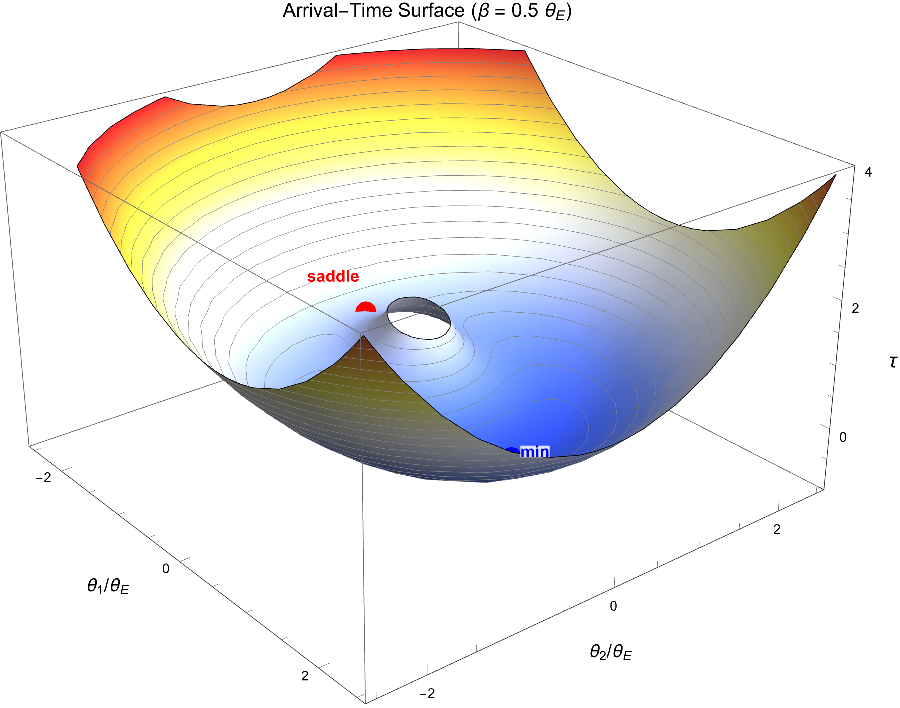
\includegraphics[width=0.85\textwidth]{../Figures/06_Fermat_Time_Delays/arrival_time_surface.pdf}
    \caption{The arrival-time surface $\tau(\theta_1, \theta_2)$ for a
    point mass lens with source at $\vecbeta = (0.5, 0)\,\thetaE$.
    The surface shows a minimum (Type~I image, blue dot) and a saddle
    point (Type~II image, red dot).  The minimum has the smaller
    arrival time and corresponds to the image that is observed first.
    The difference in $\tau$ between the two stationary points gives
    the dimensionless time delay.  Generated by
    \texttt{time\_delay\_function.wl}.}
    \label{fig:arrival_time_surface}
\end{figure}

\subsection{The Einstein Ring as a Degenerate Minimum}

When the source is exactly behind the lens ($\vecbeta = 0$), the
Fermat potential becomes circularly symmetric:
\begin{equation}
    \tau(\vectheta, \mathbf{0}) = \half|\vectheta|^2
    - \thetaE^2\, \ln|\vectheta| \,.
\end{equation}
The stationarity condition $d\tau/d|\vectheta| = 0$ gives
$|\vectheta| = \thetaE$, which is the Einstein ring.  The minimum
of $\tau$ is no longer an isolated point but a \textbf{circle} of
stationary points --- the Einstein ring is a degenerate minimum of
the arrival-time surface.

\begin{figure}[ht]
    \centering
    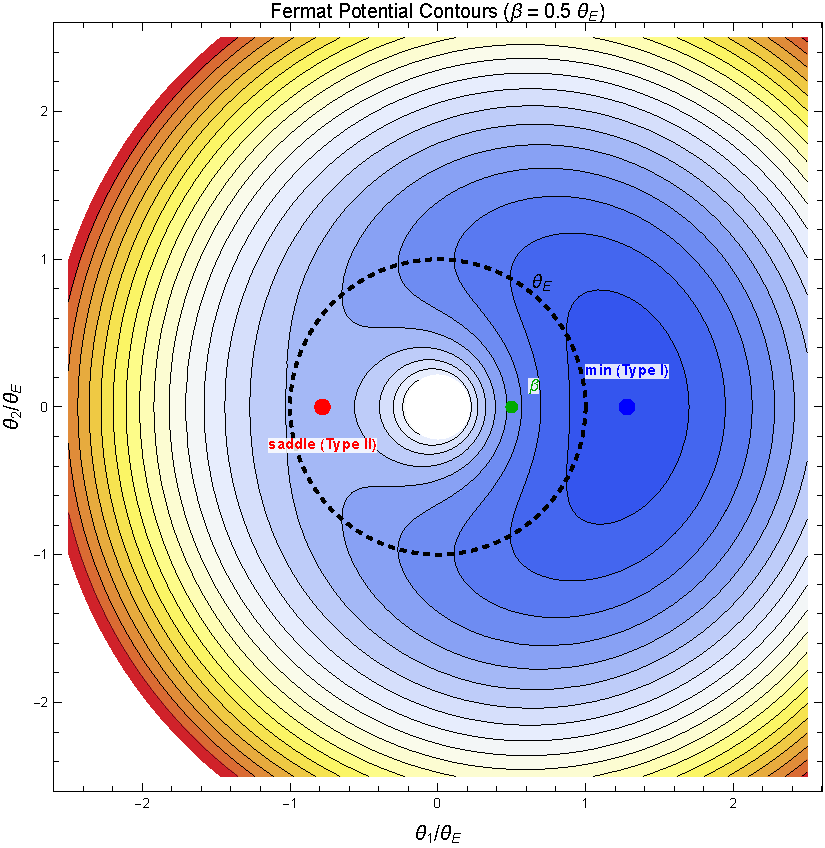
\includegraphics[width=0.78\textwidth]{../Figures/06_Fermat_Time_Delays/arrival_time_contours.pdf}
    \caption{Contour plot of the Fermat potential $\tau(\theta_1,
    \theta_2)$ for a point mass lens with $\vecbeta = (0.5, 0)\,\thetaE$.
    The two stationary points (minimum and saddle) are marked.  The
    critical curve (Einstein ring, dashed circle) is overlaid.
    Generated by \texttt{time\_delay\_function.wl}.}
    \label{fig:arrival_time_contours}
\end{figure}


% =====================================================================
\section{Observable Time Delays}
\label{sec:observable_time_delays}

The arrival time at each image $\vectheta_i$ is given by
eq.~\eqref{eq:time_delay_function}.  The \textbf{time delay} between
two images $i$ and $j$ is the difference in their arrival times:
\begin{equation}
    \boxed{
    \Delta t_{ij} = t(\vectheta_i) - t(\vectheta_j)
    = \frac{(1 + z_d)}{\speedoflight}\,
    \frac{\Dd\,\Ds}{\Dds}\,
    \left[\tau(\vectheta_i, \vecbeta) - \tau(\vectheta_j, \vecbeta)\right]
    }
    \label{eq:time_delay_between_images}
\end{equation}

This quantity is \textbf{directly observable}: if the source is variable
(as quasars are), the light curves measured at the two image positions
will show the same variability pattern, but shifted by $\Delta t_{ij}$.
By cross-correlating the light curves, one can extract $\Delta t_{ij}$
to high precision.

\begin{remark}
The time delay $\Delta t_{ij}$ depends on three ingredients:
\begin{enumerate}[nosep]
    \item The \textbf{cosmological distances} $(1+z_d)\,\Dd\,\Ds/\Dds$,
          which encode the expansion history of the universe.
    \item The \textbf{image positions} $\vectheta_i$, $\vectheta_j$,
          which are directly observed.
    \item The \textbf{lensing potential} $\psiL(\vectheta)$, which must
          be modeled from the observed lens properties (mass distribution,
          image positions, fluxes, etc.).
\end{enumerate}
Given items (2) and (3), a measurement of $\Delta t_{ij}$ constrains
the distance combination in item (1) --- and hence the cosmological
parameters.
\end{remark}


% =====================================================================
\section{Time Delay and the Hubble Constant}
\label{sec:time_delay_H0}

The key cosmological application of time delays is the measurement of
the Hubble constant $\Hubble$.  The distance combination
$\Dd\,\Ds / \Dds$ is an angular diameter distance ratio that scales
inversely with the Hubble constant:
\begin{equation}
    \frac{\Dd\,\Ds}{\Dds} \propto \frac{1}{\Hubble} \,.
    \label{eq:distance_H0_scaling}
\end{equation}
This follows from the definition of angular diameter distances in
Module~\ref{ch:cosmological_distances}: all comoving distances scale as
$\speedoflight / \Hubble$ times a dimensionless integral over the
expansion history.

Therefore, the time delay between images scales as:
\begin{equation}
    \boxed{
    \Delta t \propto \Hubble^{-1}
    }
    \label{eq:Dt_H0}
\end{equation}

This is the basis of \textbf{time-delay cosmography}: by measuring
$\Delta t$ from monitoring campaigns and modeling the lens potential
$\psiL$, one can determine $\Hubble$ \textit{independently of the
cosmic distance ladder}.  The method is sometimes called ``one-step''
distance measurement, because it converts an observed time delay
directly into a physical distance.

\begin{remark}
To extract $\Hubble$ from a time delay measurement, one needs:
\begin{enumerate}[nosep]
    \item A precise measurement of $\Delta t$ (from light curve
          monitoring of a multiply-imaged variable source).
    \item The lens and source redshifts $z_d$, $z_s$.
    \item A model for the lens mass distribution $\psiL(\vectheta)$,
          constrained by the observed image positions, fluxes, and
          extended image structure.
    \item A cosmological model (usually flat $\Lambda$CDM with $\Omegam$
          fixed) to convert the distance ratio into $\Hubble$.
\end{enumerate}
The main systematic uncertainty is the lens model degeneracy (the
``mass-sheet degeneracy''), which we will encounter in later modules.
\end{remark}

\subsection{Observational Milestones}

Time-delay cosmography has been applied to a growing number of
multiply-imaged quasars:
\begin{itemize}
    \item \textbf{Q0957+561} (Walsh, Carswell \& Weymann 1979): the first
          discovered gravitational lens.  The time delay ($\Delta t \approx
          417$~days) was measured after years of photometric monitoring.
    \item \textbf{B1608+656}: a four-image lens system with three
          independent time delays, providing strong constraints.
    \item \textbf{H0LiCOW/TDCOSMO} (2017--present): a systematic program
          combining precise time delays from COSMOGRAIL monitoring with
          detailed lens models and line-of-sight structure analysis.
          Their combined result gives $\Hubble = 73.3^{+1.7}_{-1.8}$~km\,s$^{-1}$\,Mpc$^{-1}$,
          in agreement with local distance ladder measurements and in
          some tension with the CMB value ($\Hubble \approx 67$~km\,s$^{-1}$\,Mpc$^{-1}$
          from Planck).
\end{itemize}


% =====================================================================
\section{Example: Point Mass Time Delay}
\label{sec:point_mass_time_delay}

We now compute the time delay for a point mass lens explicitly.  This
illustrative calculation demonstrates the method and gives a sense of
the physical scales involved.

\subsection{Fermat Potential for the Point Mass}

Using the lensing potential $\psiL(\vectheta) = \thetaE^2 \ln|\vectheta|$
and working in units of $\thetaE$ (i.e., defining $x = \theta/\thetaE$
and $y = \beta/\thetaE$), the Fermat potential along the symmetry axis
(where both images lie for a point mass) is:
\begin{equation}
    \tau(x) = \half(x - y)^2 - \ln|x| \,,
    \label{eq:tau_point_mass_1d}
\end{equation}
where we have set $\thetaE = 1$ in the logarithmic term.

The two image positions are $x_\pm = (y \pm \sqrt{y^2 + 4})/2$.

\subsection{Time Delay Computation}

The Fermat potential at the two images is:
\begin{align}
    \tau(x_+) &= \half(x_+ - y)^2 - \ln x_+ \,, \\
    \tau(x_-) &= \half(x_- - y)^2 - \ln|x_-| \,.
\end{align}
The dimensionless time delay is $\Delta\tau = \tau(x_-) - \tau(x_+)$
(since $\tau(x_-) > \tau(x_+)$, the saddle image arrives later).

After algebraic simplification (verified in
\mathlink{06_Fermat_Time_Delays/time_delay_function.wl}{time\_delay\_function.wl}),
the result is:
\begin{equation}
    \boxed{
    \Delta\tau = \frac{y\sqrt{y^2 + 4}}{2}
    + \ln\!\left(\frac{\sqrt{y^2 + 4} + y}{\sqrt{y^2 + 4} - y}\right)
    }
    \label{eq:delta_tau_point_mass}
\end{equation}
where $y = \beta / \thetaE$ is the dimensionless source position.

The physical time delay is:
\begin{equation}
    \Delta t = \frac{(1 + z_d)}{\speedoflight}\,
    \frac{\Dd\,\Ds}{\Dds}\, \thetaE^2\, \Delta\tau \,.
    \label{eq:delta_t_point_mass}
\end{equation}
Using $\thetaE^2 = 4\Gnewton M / (\speedoflight^2) \cdot \Dds / (\Dd\,\Ds)$:
\begin{equation}
    \Delta t = \frac{4\Gnewton M}{\speedoflight^3}\, (1 + z_d)\, \Delta\tau
    = \frac{\RS}{\speedoflight}\, (1 + z_d)\, \Delta\tau \,,
    \label{eq:delta_t_schwarzschild}
\end{equation}
where $\RS = 2\Gnewton M / \speedoflight^2$ is the Schwarzschild
radius.

\begin{example}
\label{ex:point_mass_numerical}
\textbf{Numerical time delay for a galaxy-mass point lens.}

Consider a lens mass $M = 10^{12}\,\Msun$ at $z_d = 0.3$ with a source
at $\beta = 0.5\,\thetaE$ ($y = 0.5$).  The Schwarzschild radius is:
\begin{equation*}
    \RS = \frac{2 \times 6.674 \times 10^{-11} \times
    10^{12} \times 1.989 \times 10^{30}}{(2.998 \times 10^8)^2}
    \approx 2.95 \times 10^{15}~\text{m}
    \approx 0.096~\text{pc} \,.
\end{equation*}
For $y = 0.5$: $\sqrt{y^2 + 4} = \sqrt{4.25} \approx 2.0616$.
\begin{align*}
    \Delta\tau &= \frac{0.5 \times 2.0616}{2}
    + \ln\!\left(\frac{2.0616 + 0.5}{2.0616 - 0.5}\right) \\
    &= 0.5154 + \ln(1.6401)
    = 0.5154 + 0.4947 = 1.0101 \,.
\end{align*}
The time delay is:
\begin{equation*}
    \Delta t = \frac{2.95 \times 10^{15}}{2.998 \times 10^8}
    \times 1.3 \times 1.0101
    \approx 1.29 \times 10^{7}~\text{s}
    \approx 149~\text{days} \,.
\end{equation*}
This is a realistic order of magnitude --- observed time delays in
galaxy-scale lens systems range from days to months.  Computed and
verified in
\mathlink{06_Fermat_Time_Delays/time_delay_function.wl}{time\_delay\_function.wl}.
\end{example}

\begin{figure}[ht]
    \centering
    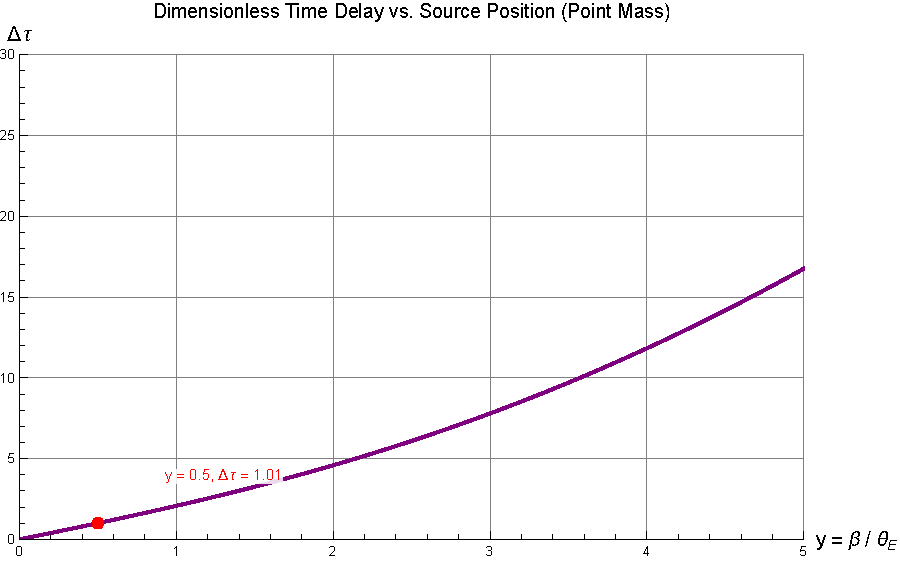
\includegraphics[width=0.78\textwidth]{../Figures/06_Fermat_Time_Delays/time_delay_vs_beta.pdf}
    \caption{Dimensionless time delay $\Delta\tau$ between the two images
    of a point mass lens as a function of the source position
    $y = \beta / \thetaE$.  The time delay increases with the source
    offset.  For $y \to 0$ (Einstein ring limit), $\Delta\tau \to 0$
    because the two images become symmetric.  Generated by
    \texttt{time\_delay\_function.wl}.}
    \label{fig:time_delay_vs_beta}
\end{figure}


% =====================================================================
\section{Example: SIS Time Delay}
\label{sec:sis_time_delay}

As a preview for Module~7 (axially symmetric lens models), we state the
time delay for the \textbf{singular isothermal sphere} (SIS).  The SIS
is characterized by its velocity dispersion $\sigma_v$, and its Einstein
radius is $\thetaE = 4\pi\,(\sigma_v/\speedoflight)^2\,\Dds/\Ds$.

For a source inside the Einstein ring ($\beta < \thetaE$), the SIS
produces two images at positions $\theta_\pm = \beta \pm \thetaE$
(both on the same side of the lens for $\theta_+$, opposite for
$\theta_-$).  The lensing potential is
$\psiL(\vectheta) = \thetaE\,|\vectheta|$, and the time delay between
the two images is:
\begin{equation}
    \boxed{
    \Delta t_{\mathrm{SIS}} = \frac{(1 + z_d)}{\speedoflight}\,
    \frac{\Dd\,\Ds}{\Dds}\,
    \frac{\thetaE^2}{2}\left(
    \frac{\theta_+^2 - \theta_-^2}{\thetaE^2}
    \right)
    = \frac{(1 + z_d)}{2\speedoflight}\,
    \frac{\Dd\,\Ds}{\Dds}\,
    \left(\theta_+^2 - \theta_-^2\right)
    }
    \label{eq:time_delay_SIS}
\end{equation}
Since $\theta_+^2 - \theta_-^2 = (\theta_+ + \theta_-)(\theta_+ - \theta_-)
= 2\beta \cdot 2\thetaE = 4\beta\,\thetaE$, this simplifies to:
\begin{equation}
    \Delta t_{\mathrm{SIS}} = \frac{2(1 + z_d)}{\speedoflight}\,
    \frac{\Dd\,\Ds}{\Dds}\, \beta\,\thetaE \,.
    \label{eq:time_delay_SIS_simple}
\end{equation}
For the SIS, the time delay is proportional to the source position ---
the further the source from the optical axis, the larger the time delay.
This simple relation makes the SIS a useful ``first approximation'' for
time-delay estimates.


% =====================================================================
\section{Summary}
\label{sec:fermat_summary}

\begin{itemize}
    \item The \textbf{time delay function}
          $t(\vectheta) \propto \tau(\vectheta, \vecbeta)$
          gives the arrival time of a photon passing through the lens
          plane at $\vectheta$.  The \textbf{Fermat potential}
          $\tau = \half|\vectheta - \vecbeta|^2 - \psiL(\vectheta)$
          combines the geometric delay (extra path length) and the
          Shapiro delay (gravitational time delay from the lensing
          potential).

    \item \textbf{Fermat's principle}: images form at stationary points
          of $\tau(\vectheta)$.  The condition $\nabla_{\vectheta}\tau = 0$
          recovers the lens equation
          $\vecbeta = \vectheta - \nabla\psiL = \vectheta - \vecalpha$.

    \item Images are classified by \textbf{Morse theory}:
          \textbf{Type~I} (minimum, positive parity, arrives first),
          \textbf{Type~II} (saddle, negative parity),
          \textbf{Type~III} (maximum, positive parity, arrives last).
          \textbf{Burke's theorem}: the number of images is always odd
          for a transparent lens.

    \item The \textbf{arrival-time surface} $\tau(\theta_1, \theta_2)$
          visualizes the image-forming process.  For a point mass lens,
          it has a minimum and a saddle point (plus a singular maximum
          at the lens center).

    \item The \textbf{time delay between images}
          $\Delta t_{ij} \propto (1+z_d)\,\Dd\Ds/\Dds \times
          [\tau(\vectheta_i) - \tau(\vectheta_j)]$
          is directly observable by monitoring variable sources.

    \item $\Delta t \propto \Hubble^{-1}$: measuring time delays and
          modeling the lens potential gives $\Hubble$ independently of
          the distance ladder.  This is \textbf{time-delay cosmography},
          implemented by programs such as H0LiCOW/TDCOSMO.

    \item For a point mass lens, the dimensionless time delay is
          $\Delta\tau = y\sqrt{y^2+4}/2 + \ln[(\sqrt{y^2+4}+y)/(\sqrt{y^2+4}-y)]$,
          where $y = \beta/\thetaE$.  The physical time delay for a
          galaxy-mass lens is of order days to months.

    \item For the SIS, $\Delta t_{\mathrm{SIS}} \propto \beta\,\thetaE$,
          a simple linear dependence on the source position.
\end{itemize}


% =====================================================================
\section{Problems}
\label{sec:fermat_problems}

\begin{exercise}
\label{ex:fermat_lens_eq}
\textbf{(Deriving the lens equation from Fermat's principle.)}
Starting from the Fermat potential
$\tau(\vectheta, \vecbeta) = \half|\vectheta - \vecbeta|^2
- \psiL(\vectheta)$:
\begin{enumerate}[label=(\alph*)]
    \item Compute the gradient $\nabla_{\vectheta}\,\tau$.
    \item Set $\nabla_{\vectheta}\,\tau = 0$ and show that this gives
          the lens equation
          $\vecbeta = \vectheta - \nabla\psiL(\vectheta)
          = \vectheta - \vecalpha(\vectheta)$.
    \item Explain physically why images form at stationary points of
          the arrival time.
\end{enumerate}
Verify with
\solnlink{06_Fermat_Time_Delays/problems\_06.wl}{problems\_06.wl}.
\end{exercise}

\begin{exercise}
\label{ex:point_mass_arrival}
\textbf{(Arrival times for a point mass lens.)}
Consider a point mass lens with Einstein radius $\thetaE = 1''$ and a
source at $\beta = 0.5\,\thetaE$.
\begin{enumerate}[label=(\alph*)]
    \item Find the two image positions $\theta_+$ and $\theta_-$.
    \item Compute the Fermat potential $\tau$ at each image position
          using $\tau(x) = \half(x - y)^2 - \ln|x|$ with $y = 0.5$,
          where $x = \theta / \thetaE$.
    \item Compute the dimensionless time delay
          $\Delta\tau = \tau(x_-) - \tau(x_+)$.
    \item For a lens mass $M = 10^{12}\,\Msun$ at $z_d = 0.3$, compute
          the physical time delay $\Delta t$ in days.
\end{enumerate}
Verify with
\solnlink{06_Fermat_Time_Delays/problems\_06.wl}{problems\_06.wl}.
\end{exercise}

\begin{exercise}
\label{ex:typeI_first}
\textbf{(Type~I image arrives first.)}
For a point mass lens with source at $\beta > 0$:
\begin{enumerate}[label=(\alph*)]
    \item Show that $\tau(\theta_+) < \tau(\theta_-)$, i.e., the
          minimum-image (Type~I) has a smaller value of $\tau$ than the
          saddle-image (Type~II).
    \item Verify this by computing $\tau(\theta_\pm)$ for
          $\beta = 0.1, 0.5, 1.0, 2.0$ (in units of $\thetaE$) and
          checking that $\tau(\theta_+) < \tau(\theta_-)$ in all cases.
    \item Explain why this implies the Type~I image arrives
          \textit{before} the Type~II image.
\end{enumerate}
Verify with
\solnlink{06_Fermat_Time_Delays/problems\_06.wl}{problems\_06.wl}.
\end{exercise}

\begin{exercise}
\label{ex:H0_from_time_delay}
\textbf{(Measuring $\Hubble$ from time delays.)}
A multiply-imaged quasar has a measured time delay $\Delta t = 420$~days
between two images.  The lens model gives a dimensionless Fermat
potential difference of $\tau_1 - \tau_2 = 25~\text{arcsec}^2$.  The
lens is at $z_d = 0.3$ and the source is at $z_s = 1.0$.
\begin{enumerate}[label=(\alph*)]
    \item Using the relation
          $\Delta t = (1+z_d)/\speedoflight \times \Dd\Ds/\Dds
          \times (\tau_1 - \tau_2)$,
          solve for $\Dd\Ds/\Dds$.
    \item For a flat $\Lambda$CDM cosmology with $\Omegam = 0.3$,
          show that $\Dd\Ds/\Dds \propto 1/\Hubble$ and compute the
          proportionality constant (hint: use the dimensionless distance
          ratios from Module~3).
    \item Determine $\Hubble$ in km\,s$^{-1}$\,Mpc$^{-1}$.  Compare
          with the H0LiCOW result and the Planck value.
\end{enumerate}
\textit{This is a simplified version of the analysis performed in real
time-delay cosmography.}
Verify with
\solnlink{06_Fermat_Time_Delays/problems\_06.wl}{problems\_06.wl}.
\end{exercise}

\begin{exercise}
\label{ex:arrival_surface_plot}
\textbf{(Plotting the arrival-time surface.)}
Using Mathematica (or your preferred software):
\begin{enumerate}[label=(\alph*)]
    \item Plot the arrival-time surface $\tau(\theta_1, \theta_2)$ for a
          point mass lens with source at
          $\vecbeta = (0.3, 0)\,\thetaE$.  Use $\thetaE = 1$.
    \item Identify the two stationary points on the surface.  Label them
          as ``minimum'' and ``saddle.''
    \item Make a contour plot of $\tau$ and overlay the critical curve
          (the Einstein ring $|\vectheta| = \thetaE$).
    \item Verify that the stationary points agree with the analytical
          image positions $\theta_\pm$ from the lens equation.
\end{enumerate}
See
\mathlink{06_Fermat_Time_Delays/arrival_time_surface.nb}{arrival\_time\_surface.nb}
and
\solnlink{06_Fermat_Time_Delays/problems\_06.wl}{problems\_06.wl}.
\end{exercise}
